% !TeX spellcheck = cs_CZ
%%%%%%%%%%%%%%%%%%%%%%%%%%%%%%%%%%%%%%%%%
% University Assignment Title Page 
% LaTeX Template
% Version 1.0 (27/12/12)
%
% This template has been downloaded from:
% http://www.LaTeXTemplates.com
%
% Original author:
% WikiBooks (http://en.wikibooks.org/wiki/LaTeX/Title_Creation)
%
% License:
% CC BY-NC-SA 3.0 (http://creativecommons.org/licenses/by-nc-sa/3.0/)
% 
% Instructions for using this template:
% This title page is capable of being compiled as is. This is not useful for 
% including it in another document. To do this, you have two options: 
%
% 1) Copy/paste everything between \begin{document} and \end{document} 
% starting at \begin{titlepage} and paste this into another LaTeX file where you 
% want your title page.
% OR
% 2) Remove everything outside the \begin{titlepage} and \end{titlepage} and 
% move this file to the same directory as the LaTeX file you wish to add it to. 
% Then add \input{./title_page_1.tex} to your LaTeX file where you want your
% title page.
%
%%%%%%%%%%%%%%%%%%%%%%%%%%%%%%%%%%%%%%%%%

%----------------------------------------------------------------------------------------
%	PACKAGES AND OTHER DOCUMENT CONFIGURATIONS
\documentclass[czech,12pt]{article}
\usepackage[utf8]{inputenc}
\usepackage[czech]{babel}
\usepackage{graphicx}
\usepackage{hyperref}
\usepackage{listings}
%----------------------------------------------------------------------------------------
\begin{document}

\begin{titlepage}
\newcommand{\HRule}{\rule{\linewidth}{0.5mm}} % Defines a new command for the horizontal lines, change thickness here
\center

\textsc{\LARGE Fakulta informačních technologií}\\[1.5cm] % Jmeno fakulty (university)
\textsc{\Large Paralelní architektury počítačů}\\[0.5cm] % Nazev predmetu
\textsc{\large technická zpráva}\\[0.5cm] % Druh zpravy


% TITLE
\HRule \\[0.4cm]
{ \huge \bfseries Hledání nejkratších cest v grafu}\\[0.4cm] % Nazev dokumentu (prace)
\HRule \\[1.5cm]

% AUTOR
\Large \emph{Autoři:}\\
Vojtěch \textsc{Myslivec}\\
Zdeněk \textsc{Nový}\\[2cm]	% Jmeno

% DATUM
{\large \today}\\[3cm] % Datum zmeny jako dnesek

% LOGO

\includegraphics{cvut-logo-bw.pdf}\\[1cm] % Vlozene logo (nutny balik graphicx)

\vfill % Zbytek stranky neni nic
\end{titlepage}

%--- Abstrakt ---
\renewcommand\abstractname{\begin{flushright}\begin{LARGE}\textbf{Abstrakt}\end
{LARGE}\end{flushright}}
\newcommand{\keywords}[1]{\vspace{0.8cm}\textbf{Klíčová slova\hspace{0.2cm}} #1}
\noindent\makebox[\linewidth]{\rule{\textwidth}{0.4pt}}
\begin{abstract}
Účelem této práce je sumarizovat výsledky měření řešení problému hledání nejkratších cest v grafu (NCG). Práce se zaměřuje na řešení problému Dijkstrovým a Floyd-Warshallovým algoritmem a porovnání sekvenční a několika paralelních implementací.
\end{abstract}

% --- Klicova slova ---
\keywords{Dijkstra, Floyd, Warshall, nejkratší cesty, NCG, OpenMP, Cuda}

\clearpage


%-------------------------------
%---		   Uvod		 	 ---
%-------------------------------
\section{Úvod}
Tato práce se zabývá implementací dvou algoritmů hledání nejkratších cest v grafu. Jedná se o implementaci sekvenčním algoritmem, který je poté paralelizován pro procesor a pro grafickou kartu. Pro jednotlivé algoritmy je provedeno měření, které si klade za cíl určit zrychlení paralelních algoritmů proti sekvenčnímu.

%-------------------------------
%---			NCG			 ---
%-------------------------------
\section{Hledání nejkratších cest v grafu} \label{ncg}
\subsection{Definice} \label{l:clondike:ncgdef}
Hledání nejkratších cest v grafu je NP-úplná grafová úloha, jejímž cílem je nalézt v zadaném grafu nejkratší cesty mezi všemi možnými dvojicemi uzlů A a B \cite{w:ncg}.

\subsection{Algoritmy}
\subsubsection{Dijkstrův algoritmus}
Dijkstrův algoritmus slouží k nalezení všech nejkratších cest ze zadaného uzlu do všech ostatních uzlů grafu. Graf nesmí obsahovat hrany se zápornou délkou \cite{w:dij:def}.

\paragraph{Princip}
Dijkstrův algoritmus je zobecněné prohledávání grafu do šířky, při kterém se vlna šíří na základě vzdálenosti od zdrojového uzlu. K uchovávání uzlů slouží prioritní fronta, která je řazena podle vzrůstající vzdálenosti od zdroje. V každém kroku algoritmu je vybrán uzel s nejmenší vzdáleností a pro každého souseda je vypočítána jeho vzdálenost od zdrojového uzlu \cite{w:dij:def}.

\subsubsection{Floyd-Warshallův algoritmus}
Floyd-Warshallův algoritmus slouží k nalezení nejkratších cest mezi všemi dvojicemi uzlů v grafu. Graf může obsahovat hrany, ale nikoliv cykly, záporné délky \cite{w:fw:def}.

\paragraph{Princip} \label{l:fw:princip}
Floyd-Warhsallův algoritmus pracuje s maticí sousednosti, kde hrana je ohodnocena vahou. Na počátku tato matice obsahuje pouze vzdálenosti dvou uzlů, mezi kterými je vedena hrana. V každém kroku je vybrán jeden uzel jako prostředník. Prvek matice sousednosti se přepočítá, pokud je vzdálenost z počátečního do koncového uzlu kratší přes nového prostředníka než bez něj \cite{w:fw:def}.


%-------------------------------
%---		Sekvencni		 ---
%-------------------------------
\section{Sekvenční algoritmus}
\subsection{Společná implementace}
Oba algoritmy vycházejí z obecněho principu, který je popsán v kapitole \ref{l:fw:princip}. Algoritmy pracují s grafem, který je programu předložen jako soubor, ve kterém je graf ve formě matice sousednosti. Společnou částí je tedy načítání vstupu a jeho kontrola.

\subsection{Dijkstrův algoritmus}
Protože Dijkstrův algoritmus slouží k hledání nejkratších cest od jednoho zdrojového uzlu, je nutné jej spouštět pro každý uzel grafu. To zajišťuje funkce \textit{dijkstraNtoN}.

\subsubsection{Dijkstrův algoritmus z jednoho zdroje}
Pro výpočet Dijkstrova algoritmu z jednoho zdrojového uzlu se alokují tři pole o velikosti počtu uzlů. V jednom je uložena vzdálenost daného uzlu od zdrojového, ve druhém předchozí uzel v nalezené nejkratší cestě. Třetí pole určuje, jestli je už uzel uzavřený pro výpočty.

Algoritmus prochází postupně, podle nejmenší vzdálenosti, všechny uzly, které se nacházejí v prioritní frontě. Z daného uzlu vypočítá pro každého svého souseda novou cestu, která by vedla přes uzel samotný a porovná ji s dosavadní vzdáleností souseda. Menší vzdálenost je zapsána do pole vzdáleností a algoritmus pokračuje.

\paragraph{Prioritní fronta} \label{l:dij:fron}
Za účelem prioritní fronty byla implementována binární halda, kde složitost výběru minima je logaritmická, oproti nativní implementaci pomocí pole, kde je složitost výběru minima lineární.


\subsection{Floyd-Warshallův algoritmus}
Floyd-Warshallův algoritmus obsahuje tři vnořené for cykly a funguje na principu popsaném v \ref{l:fw:princip}. Jako datové struktury používá čtyři pole o velikosti počtu uzlů. Pro každý uzel si algoritmus udržuje aktuální vzdálenosti ke všem uzlům a navíc vzdálenosti z předchozí iterace. Další dvě pole obsahují předchozí uzel v nalezené cestě. 

\subsection{Implementace}
Aktuální implementace je k nahlédnutí i ke stažení na adrese \url{https://github.com/VojtechMyslivec/PAP-NCG}. Sekvenční algoritmus se nachází ve složce \textit{01\_sekvencni}.


%-------------------------------
%---		OpenMP			 ---
%-------------------------------
\section{Paralelní algoritmus pomocí knihovny OpenMP}
\subsection{Dijkstrův algoritmus}
Paralelizace algoritmu spočívá v paralelizaci cyklu, který prochází jednotlivé uzly a pro ně řeší problém hledání nejkratší cesty v grafu z jednoho počátečního uzlu. Každé vlákno tedy zpracovává jeden uzel jako počáteční a z něj hledá nejkratší cesty do všech ostatních uzlů.

\subsubsection{Paměťové struktury}
Každé vlákno dostane ukazatel na strukturu grafu. Protože všechna vlákna používají strukturu grafu pouze ke čtení, nedochází při přístupu k této struktuře k žádným problémům.

Každé vlákno si vytvoří jeden objekt, ve kterém si alokuje vlastní pole vzdáleností a předchůdců, které používá pro své výpočty. Tyto struktury jsou po ukončení funkce vlákna dealokovány společně s objektem.

\subsubsection{Úprava algoritmu}
Z důvodu paralelizace algoritmu bylo nutné upravit použitou prioritní frontu. V sekvenčním řešení byla použita implementace pomocí binární haldy \ref{l:dij:fron}. Z důvodu paralelizace výběru minima z fronty je pro paralelní řešení výhodnější použít implementaci polem.


\subsubsection{Vektorizace}


\subsubsection{Optimalizace}


\subsection{Floyd-Warshallův algoritmus}
Díky třem vnořeným sekvenčního algoritmu existuje několik možností, jak algoritmus paralelizovat.

\subsubsection{První varianta}
První variantou je algoritmus paralelizovat pouze v jednom cyklu, který definuje, která řádka je právě zpracovávána. Přidělená data jednomu vláknu zobrazuje obrázek \ref{f:flo:omp}. Algoritmus zapisuje pouze do přidělených sloupců, tedy řádků zobrazených v části \textit{a}. Řádek \textit{k} v části \textit{b} využívají všechna vlákna pouze ke čtení, proto zde nedochází ke konfliktům. Tato varianta je implementována.

\begin{figure}
    \centering
    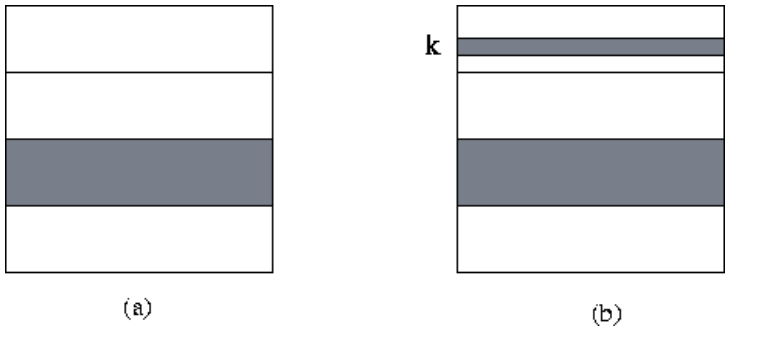
\includegraphics[width=\textwidth]{floyd-openmp}
    \caption{Ukázka dat přidělených jednomu vláknu při paralelizaci jednoho cyklu \cite{w:flo:omp}.}
    \label{f:flo:omp}
\end{figure}


\subsubsection{Druhá varianta}
Druhou variantou, jak problém paralelizovat je použít původní variantu a přidat paralelizaci zároveň ve vnitřním cyklu, který prochází jednotlivé sloupce matice. V takovém případě by jednomu vláknu byl přidělen jeden nebo více necelých řádků ohraničených sloupci. Tato varianta se jeví vhodnější pouze při velkém počtu dostupných vláken, proto není v naší implementaci použita.

\subsubsection{Vektorizace}

\subsubsection{Optimalizace}

\subsection{Měření}
Na obou algoritmech bylo provedeno měření, které si klade za cíl analyzovat čas, zrychlení a efektivitu použitého paralelního algoritmu. Měření bylo prováděno na hustých grafech, kde při generování grafů byla použita pravděpodobnost 0.5, že mezi dvěmi uzly existuje hrana.

\subsubsection{Testovací data}
Jako testovací data byly vygenerovány grafy s počtem uzlů 1000, 2000, 3000, 4000, 5000. Měření probíhalo na serveru \url{star2.fit.cvut.cz} na stroji \textit{gpu-02} pro počet vláken 1, 2, 4, 6, 8, 12, 24.

\subsubsection{Výsledky}
Grafy \ref{f:mer:cas}, \ref{f:mer:zry} a \ref{f:mer:efe} ukazují výsledky měření z pohledu času, zrychlení a efektivity.

% Cas
\begin{figure}
    \centering
    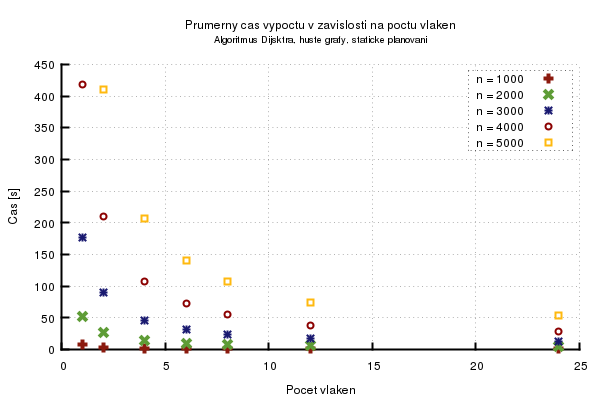
\includegraphics[width=0.45\textwidth]{../grafy/02_openMP/02-01-Dijsktra_cas}
    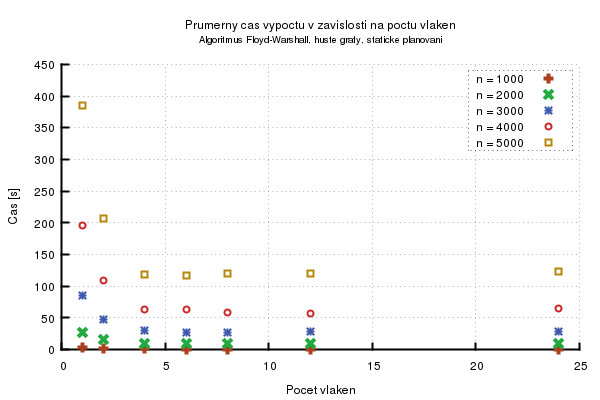
\includegraphics[width=0.45\textwidth]{../grafy/02_openMP/02-01-Floyd_cas}
    \caption{Závislost průměrného času výpočtu v závislosti na počtu vláken za použití statického plánování.}
    \label{f:mer:cas}
\end{figure}

% Zrychleni
\begin{figure}
    \centering
    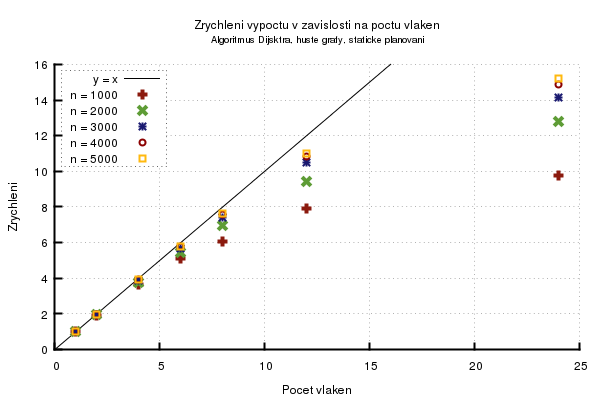
\includegraphics[width=0.45\textwidth]{../grafy/02_openMP/02-02-Dijsktra_zrychleni}
    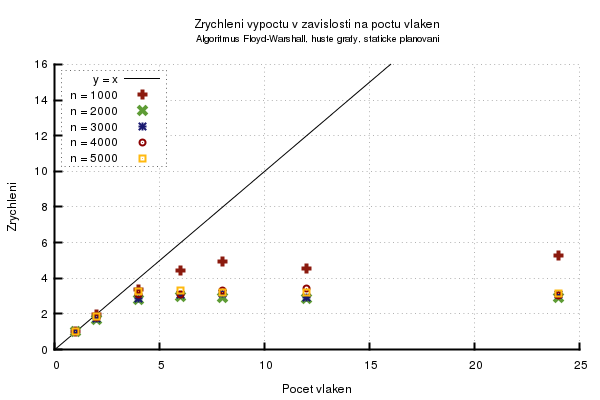
\includegraphics[width=0.45\textwidth]{../grafy/02_openMP/02-02-Floyd_zrychleni}
    \caption{Závislost zrychlení paralelního algoritmu oproti sekvenčnímu v závislosti na počtu vláken za použití statického plánování.}
    \label{f:mer:zry}
\end{figure}

% Efektivita
\begin{figure}
    \centering
    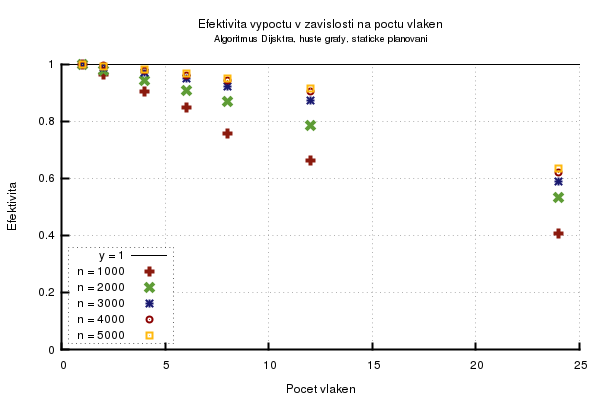
\includegraphics[width=0.45\textwidth]{../grafy/02_openMP/02-03-Dijsktra_efektivita}
    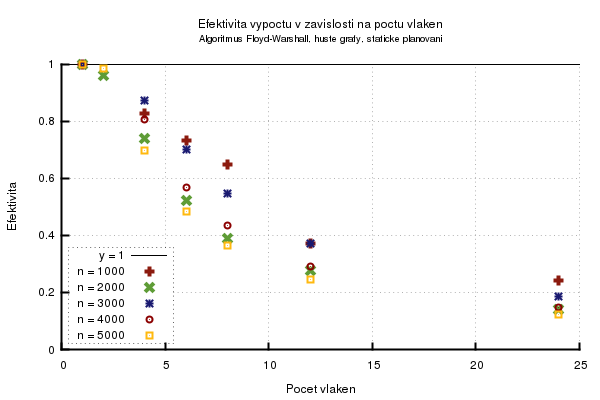
\includegraphics[width=0.45\textwidth]{../grafy/02_openMP/02-03-Floyd_efektivita}
    \caption{Závislost efektivity algoritmu v závislosti na počtu vláken za použití statického plánování.}
    \label{f:mer:efe}
\end{figure}

\subsubsection{Analýza}
\paragraph{Dijsktra}
U výpočetního času je z grafů \ref{f:mer:cas} je patrná exponenciální závislost, kdy se čas pro větší počet vláken téměř nezkracuje. Zrychlení, které je zobrazeno v grafu \ref{f:mer:zry} na počátku stoupá téměř lineárně a teprve pro velký počet vláken se zrychlení zmírňuje a křivka dostává logaritmický tvar. Z výše uvedeného vyplývá efektivita, která je zobrazena v grafu \ref{f:mer:efe}.

\paragraph{Floyd-Warshallův algoritmus}
U Floyd-Warshallova algoritmu se výpočetní čas pro počty vláken větší než 2 téměř nezkracuje. Zrychlení je tedy patrné pouze při použití 2 případně 4 vláknech. Z výše uvedené plyne, že efektivita paralelního algoritmu velmi rychle klesá.

\subsubsection{Zhodnocení}
Efektivita Dijkstrova algoritmu s přidáváním vláken pomalu klesá a například pro 24 vláken dosahuje hodnoty 0.5. Naproti tomu u Floyd-Warshallova algoritmu klesá efektivita mnohem rychleji a na hodnotě 0.5 se nachází už pro 6 vláken. 

Výrazně lépe ve prospěch Dijkstrova paralelního algoritmu vycházejí i ostatní ukazatele -- zrychlení a čas výpočtu.

Výsledky Floyd-Warshallova algoritmu mohou být způsobeny opakovaným vytvářením a rušením vláken. V každém vnějším cyklu se vytvoří daný počet vláken, zpracuje jeden uzel a všechna tato vytvořená vlákna se opět ukončí. Tedy za běhu algoritmu se vytváří a ruší \textit{pocet\_uzlu * vlaken}, kde parametr \textit{vlaken} je počet najednou vytvářených paralelních vláken.


%-------------------------------
%---		CUDA			 ---
%-------------------------------
%\section{Paralelní algoritmus pomocí technologie CUDA}
%\subsection{Dijkstrův algoritmus}
%\subsubsection{Úprava algoritmu}
%\subsubsection{Optimalizace}
%
%\subsection{Floyd-Warshallův algoritmus}
%\subsubsection{Úprava algoritmu}
%\subsubsection{Optimalizace}
%
%\subsection{Měření}
%\subsubsection{Analýza}
%\subsubsection{Zhodnocení}
%
%
%\section{Závěr}








\clearpage
\bibliographystyle{czechiso} % nutny soubor czechiso.bst
\bibliography{citace}

\end{document}